%本项目遵循MIT License (MIT)
%基于 中文技术报告Latex模板(单栏)_CJC_XeLaTeX 更改，用于广东石油化工学院的非官方学报XeLatex模板，在视觉上做到了大致一致。

%参考文献遵循GB/T 7741-2015标准

%https://www.overleaf.com/latex/templates/zhong-wen-ji-zhu-bao-gao-latexmo-ban-dan-lan-cjc-xelatex/tcnttxfsqykx

% LiuYi YU 2026/04/25 Ver.0.1

%本项目GitHub链接 https://github.com/LiuyiRigel/GDUPT-Journal

%The MIT License (MIT)
%Copyright © 2026 <copyright holders>

%Permission is hereby granted, free of charge, to any person obtaining a copy of this software and associated documentation files (the “Software”), to deal in the Software without restriction, including without limitation the rights to use, copy, modify, merge, publish, distribute, sublicense, and/or sell copies of the Software, and to permit persons to whom the Software is furnished to do so, subject to the following conditions:

%The above copyright notice and this permission notice shall be included in all copies or substantial portions of the Software.

%THE SOFTWARE IS PROVIDED “AS IS”, WITHOUT WARRANTY OF ANY KIND, EXPRESS OR IMPLIED, INCLUDING BUT NOT LIMITED TO THE WARRANTIES OF MERCHANTABILITY, FITNESS FOR A PARTICULAR PURPOSE AND NONINFRINGEMENT. IN NO EVENT SHALL THE AUTHORS OR COPYRIGHT HOLDERS BE LIABLE FOR ANY CLAIM, DAMAGES OR OTHER LIABILITY, WHETHER IN AN ACTION OF CONTRACT, TORT OR OTHERWISE, ARISING FROM, OUT OF OR IN CONNECTION WITH THE SOFTWARE OR THE USE OR OTHER DEALINGS IN THE SOFTWARE.
%===============================%

\documentclass[10.5pt,compsoc,UTF8]{CjC}
\usepackage{CTEX}
\usepackage{graphicx}
\usepackage{footmisc}
\usepackage{subfigure}
\usepackage{url}
\usepackage{multirow}
\usepackage{multicol}
\usepackage[noadjust]{cite}
\usepackage{amsmath,amsthm}
\usepackage{amssymb,amsfonts}
\usepackage{booktabs}
\usepackage{color}
\usepackage{ccaption}
\usepackage{booktabs}
\usepackage{float}
\usepackage{fancyhdr}
\usepackage{caption}
\usepackage{xcolor,stfloats}
\usepackage{comment}
\setcounter{page}{1}
\graphicspath{{figures/}}
\usepackage{cuted}%flushend,
\usepackage{captionhack}
\usepackage{epstopdf}
\usepackage{gbt7714}

%===============================%



\headevenname{\mbox{\quad} \hfill  \mbox{\zihao{-5}{ \hfill 《课程名称》  } \hspace {0mm} \mbox{2023 年 9 月}}}%
\headoddname{作者姓名等 \hfill 报告题目}%

%footnote use of *
\renewcommand{\thefootnote}{}
\setcounter{footnote}{0}
\renewcommand\footnotelayout{\zihao{5-}}

\newtheoremstyle{mystyle}{0pt}{0pt}{\normalfont}{1em}{\bf}{}{1em}{}
\theoremstyle{mystyle}
\renewcommand\figurename{figure~}
\renewcommand{\thesubfigure}{(\alph{subfigure})}
\newcommand{\upcite}[1]{\textsuperscript{\cite{#1}}}
\renewcommand{\labelenumi}{(\arabic{enumi})}
\newcommand{\tabincell}[2]{\begin{tabular}{@{}#1@{}}#2\end{tabular}}
\newcommand{\abc}{\color{white}\vrule width 2pt}
\renewcommand{\bibsection}{}
\makeatletter
\renewcommand{\@biblabel}[1]{[#1]\hfill}
\makeatother
\setlength\parindent{2em}
%\renewcommand{\hth}{\begin{CJK*}{UTF8}{gbsn}}
%\renewcommand{\htss}{\begin{CJK*}{UTF8}{gbsn}}
\renewcommand{\familydefault}{\rmdefault}  % 确保宋体
\zihao{5}

\begin{document}
\zihao{5}
\songti

\hyphenpenalty=50000
\makeatletter
\newcommand\mysmall{\@setfontsize\mysmall{7}{9.5}}
\newenvironment{tablehere}
  {\def\@captype{table}}

\let\temp\footnote
\renewcommand \footnote[1]{\temp{\zihao{-5}#1}}


\thispagestyle{plain}%
\thispagestyle{empty}%
\pagestyle{plain}

% \begin{table*}[!t]
\vspace {-13mm}

{
\centering

{\zihao{2-} \heiti 石化设备防腐信息管理系统 }

\vskip 5mm

{\zihao{4-}\kaishu 作者名$^{1}$\quad  作者名$^{2}$ \quad 作者名$^{3 }$}

\footnote{\raggedright\noindent
\noindent {\zihao{5-}\heiti 收稿日期：} {\zihao{5-} yyyy-mm-dd;} \\
\noindent {\zihao{5-}\heiti 基金项目：} {\zihao{5-} 项目名称（编号）；项目名称（编号）} \\
\noindent {\zihao{5-}\heiti 作者简介：} {\zihao{5-} 名字（出生年—），性别，籍贯，学历，学位，职称，硕导（博导），主要研究方向为}
}


\zihao{5-}{(1.广东石油化工学院 文法学院，广东 茂名，525000；2.广州大学 人文学院，广州 51000)}

}

\vskip 5mm

\zihao{5-}{
\setlength{\baselineskip}{16pt}\selectfont{
\noindent {\heiti 摘要: }{\fangsong
内容小五号仿宋}
\par}}


\vspace {2mm}

\zihao{5-}{\noindent
{\heiti 关键词：}{\fangsong
系统方法；电路教学；工程实践}
}


\noindent
\begin{tabular}{@{}p{0.3\textwidth}@{}p{0.3\textwidth}@{}p{0.3\textwidth}@{}}
{\zihao{5-}\heiti 中图分类号：} {\zihao{5-}\songti 内容} &
\centering {\zihao{5-}\heiti 文献识别号：} {\zihao{5-}\songti 内容} &
\raggedleft {\zihao{5-}\heiti 文章编号：} {\zihao{5-}\songti 内容} \\
\end{tabular}


\vskip 7mm

\zihao{5}

% \begin{multicols}{1}

%%%%%%%%%%%%%%%%%%%%%%%%%%%%%%%%%%%%%%%%%%


\section{\heiti 技术报告的基本要求}

\subsection{一般学术论文的撰写要求}

研究性论文主体应包括引言(重点论述研究的科学问题、意义、解决思路、价值、贡献等)、相关工作(为与引言部分独立的一个章节)、主要成果论述、关键实现技术、验证(对比实验或理论证明)、结论(结束语)等内容；系统实现或实验应有关键点的详细论述，以便读者能够重复实现论文所述成果。实验应有具体的实验环境设置、全面细致的数据对比分析。


%%%%%%%%%%%%%%%%%%%%%%%%%%%%%%%%%%%%%%%%%%
%%%%%%%%%%%%%%%%%%%%%%%%%%%%%%%%%%%%%%%%%%

\subsection{插图格式}


\begin{figure}[htbp]
\centering
\centerline{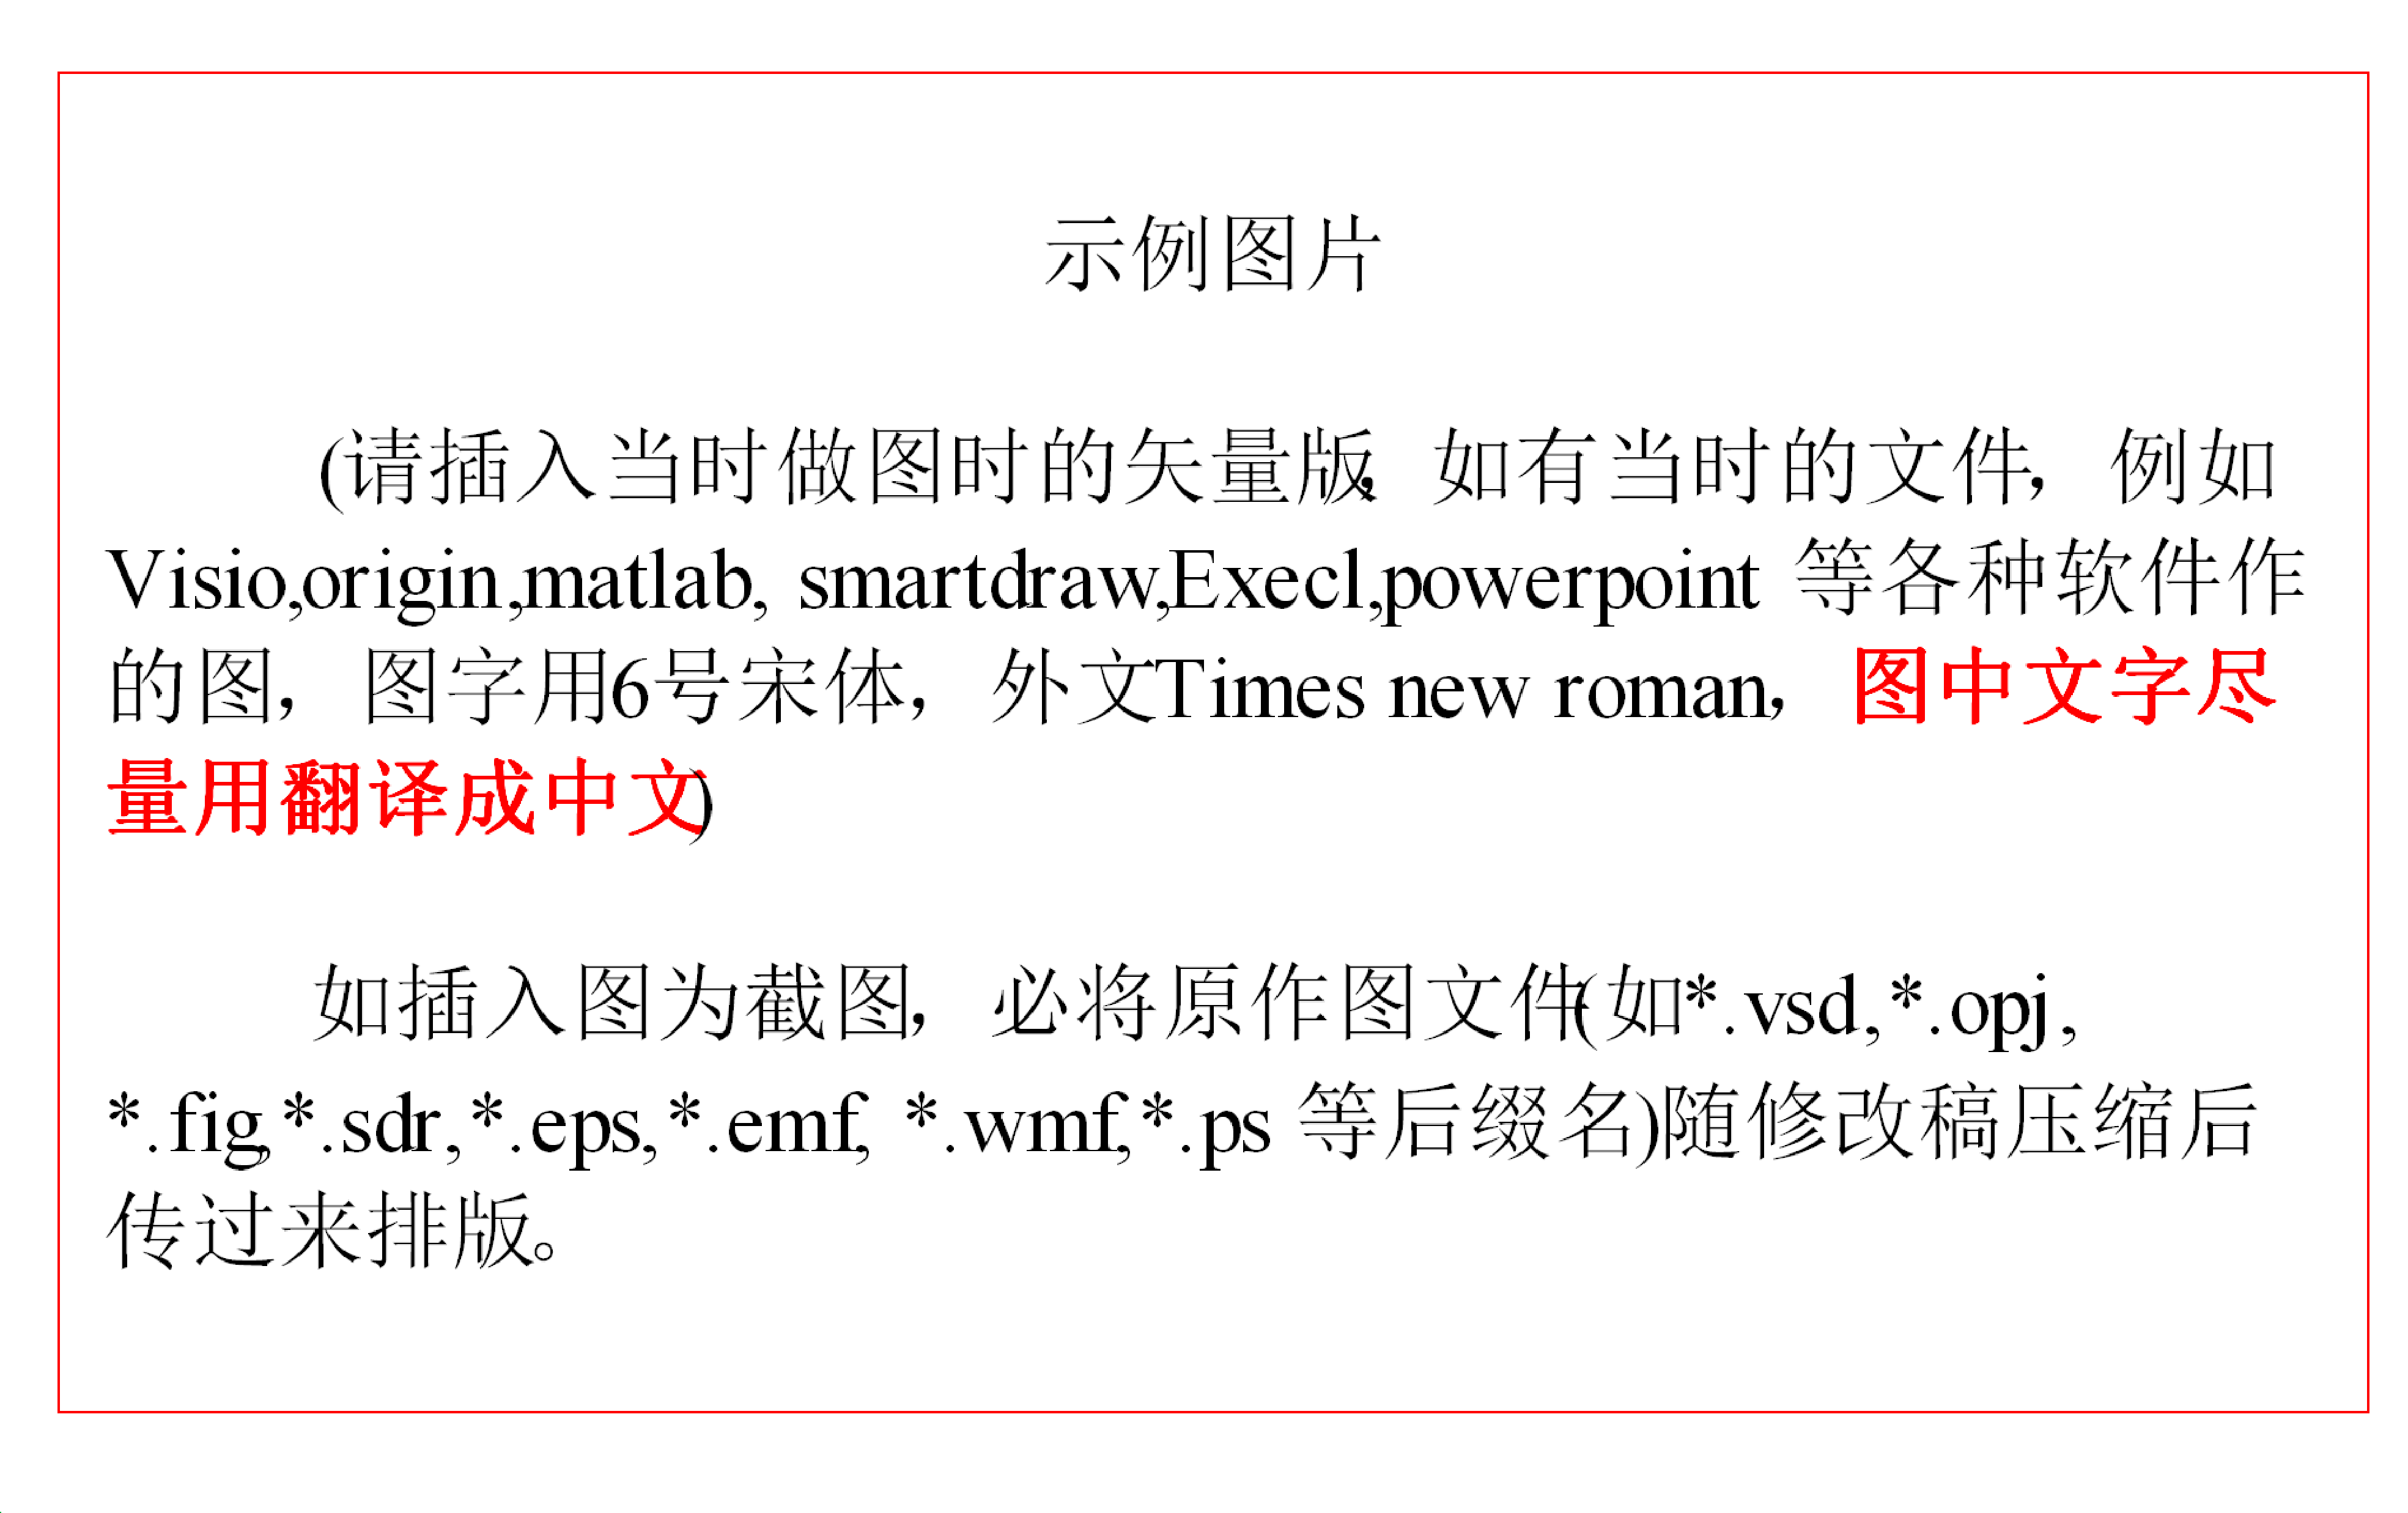
\includegraphics[width=0.6\linewidth]{CJC1.pdf}}
\heiti 图X\quad  图片说明 *字体为小5号，图中的子图要有子图说明*
\label{fig1}
\end{figure}


%%%%%%%%%%%%%%%%%%%%%%%%55

\newpage

\subsection{表格格式}

\begin{table}[htbp]
\centering {\songti 表X\quad 表说明 *表说明采用黑体*}
% \caption{表说明 *表说明采用黑体*}
\vspace {-2.5mm}
\begin{center}
\begin{tabular}{ll}
\toprule
*示例表格*&*第1行为表头,表头要有内容* \\
\hline
&
 \\
&
 \\
&
 \\
&
 \\
\bottomrule
\end{tabular}
\label{tab1}
\end{center}
\end{table}



%%%%%%%%%%%%%%%%%%%%%%%%%%%%%%%%%%%%%%%5
%%%%%%%%%%%%%%%%%%%%%%%%%%%%%%%%%%%%%%%%%

\subsection{参考文献}
这是参考文献示例。参考文献应遵循GB/T 7741-2015标准。引用文献1~\cite{Bohan1928}，文献2~\cite{chen1980zhongguo}，文献3-5~\cite{bravo1990comparative,niu2013zonghe,yuan2012lana}。

%%%%%%%%%%%%%%%%%%%%%%%%%%%%%%%%
%%%%%%%%%%%%%%%%%%%%%%%%%%%%%%%%


\vspace {10mm}
\zihao{5}{
\noindent \textsf{致\quad 谢}\quad {致谢}}

\vspace {10mm}

\centerline
{\zihao{4-}\textsf{[参考文献]}}
\zihao{5-} \addtolength{\itemsep}{-1em}


\vspace {1.5mm}
\bibliographystyle{gbt7714-numerical}
\bibliography{ref.bib}


\vspace {10mm}

\newpage

\begin{center}
\zihao{4}{ \heiti Title }\\
\vspace {5mm}

{\zihao{5}\songti YU Liuyi $^{1}$, YU Liuyi $^{2}$, YU Liuyi $^{3 }$}

\zihao{5-}{(1.Guangdong University of Petrochemical Technology, Maoming 525000, China; 2.……)}


\end{center}

\zihao{5-}{
\setlength{\baselineskip}{18pt}\selectfont{
{\bf Abstract:}
字体为Times new Roman,字号5号* 
\zihao{5-}{\noindent Do not modify the amount of space before and after the artworks. One- or two-column format artworks are preferred. and Tables, create a new break line and paste the resized artworks where desired. Do not modify the amount of space before and after the artworks. One- or two-column format artworks are preferred. All Schemes, Equations, Figures, and Tables should be mentioned in the text consecutively and numbered with Arabic numerals, and appear below where they are mentioned for the first time in the main text. To insert Schemes, Equations, Figures, and Tables, create a new break line and paste the resized artworks where desired. Do not modify the amount of space before and after the artworks. One- or two-column format artworks are preferred.Do not modify the amount of space before and after the artworks. One- or two-column format artworks are preferred. and Tables, create a new break line and paste the resized artworks where desired. 
\par}}

\vspace {2mm}

{{\bf Keywords:}
key word; key word; key word\par}}

\end{document}


